\subsubsection{Numerical experiments - Estimation of $\tau$}

\textbf{Smooth case.} We consider as a domain for \eqref{eq:OneDModel} the interval $D = \left[-1,1\right]$, final time $T = 5$ and the following functions
\begin{align}\label{eq:FunctionsOneDSmooth}
\begin{split}
	f(x) &= -V'(x), \text{ where } V(x) = 0.1(8x^4 - 8x^2 + x + 2), \\
	g(x) &= \sigma = 3.
\end{split}
\end{align}
We approximate the value of $\tau$ with a Montecarlo simulation of $\tau_h^d$ and $\tau_h^c$ computed as in \eqref{eq:TauDEM} and \eqref{eq:TauCEM} from the solutions provided by DEM and CEM respectively. In order to verify the order of convergence of the methods, we let $N$ vary in the set $2^i,i=3,\dots,12$ and we fix the number of trajectories $M$ to $10000$. In this way, the error caused by the Montecarlo estimation should not spoil the order of convergence. In Figure \ref{fig:OrdersOneD} we show the errors obtained fixing $X_0 = 0$ in both the cases of killing and reflecting boundary conditions in $x = 1$. Moreover, in Figure \ref{fig:ApproxOneD} we show an approximation of $\tau$ obtained with the two methods with $h = T/128$ and $M = 1000$ for a set of 10 initial values equispaced along $D$. It is possible to remark that computing the probability of exit between two consecutive timesteps as in \eqref{eq:CEMProbHalfSpace} allows correcting the overestimation of $\tau$ obtained simply using DEM. We want to estimate the computational time for both the method. We consider $M = 10000$, killing boundary conditions and $N = 2^i, i = 3,\dots,12$. We remark that the computational time required by CEM is higher than for DEM if the same value of $h$ is employed. On the other hand, fixing the error, CEM is faster than DEM in this case.

\begin{figure}[t]
    \centering
    \begin{subfigure}{0.49\linewidth}
        \centering
        \resizebox{1\linewidth}{!}{% This file was created by matlab2tikz.
%
%The latest updates can be retrieved from
%  http://www.mathworks.com/matlabcentral/fileexchange/22022-matlab2tikz-matlab2tikz
%where you can also make suggestions and rate matlab2tikz.
%
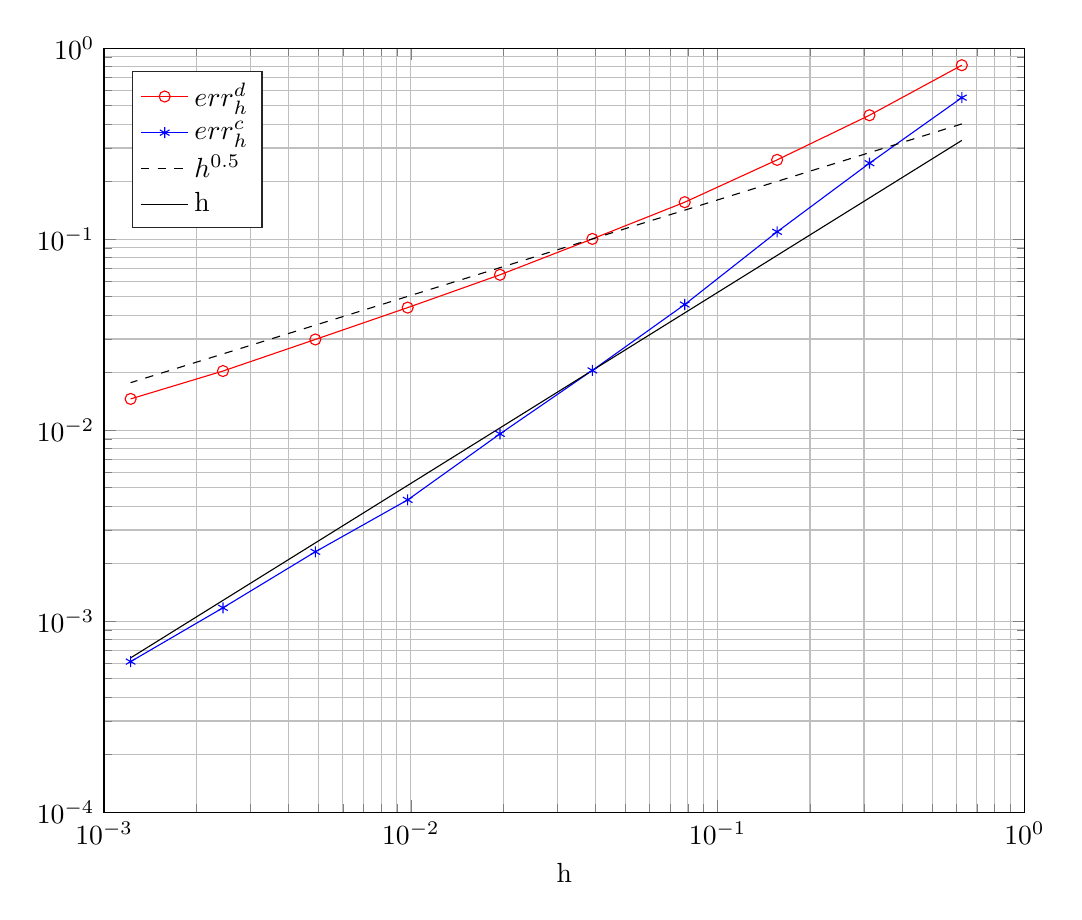
\begin{tikzpicture}

\begin{axis}[%
width=4.602in,
height=3.82in,
at={(0.772in,0.516in)},
scale only axis,
xmode=log,
xmin=0.001,
xmax=1,
xminorticks=true,
xlabel={h},
xmajorgrids,
xminorgrids,
ymode=log,
ymin=0.0001,
ymax=1,
yminorticks=true,
ymajorgrids,
yminorgrids,
axis background/.style={fill=white},
legend style={at={(0.03,0.97)},anchor=north west,legend cell align=left,align=left,draw=white!15!black}
]
\addplot [color=red,solid,mark=o,mark options={solid}]
  table[row sep=crcr]{%
0.625	0.814121166527388\\
0.3125	0.445308666527388\\
0.15625	0.260074291527388\\
0.078125	0.156160229027388\\
0.0390625	0.100300854027388\\
0.01953125	0.0650840571523877\\
0.009765625	0.0438213618398876\\
0.0048828125	0.0298496821523877\\
0.00244140625	0.0203989985586377\\
0.001220703125	0.0145757563711377\\
};
\addlegendentry{$\text{err}_\text{h}^\text{d}$};

\addplot [color=blue,solid,mark=asterisk,mark options={solid}]
  table[row sep=crcr]{%
0.625	0.550496166527388\\
0.3125	0.249839916527388\\
0.15625	0.109277416527388\\
0.078125	0.0454727290273877\\
0.0390625	0.0205547602773877\\
0.01953125	0.00956257277738766\\
0.009765625	0.00431550246488765\\
0.0048828125	0.00230768996488766\\
0.00244140625	0.00117487746488766\\
0.001220703125	0.000614086449262655\\
};
\addlegendentry{$\text{err}_\text{h}^\text{c}$};

\addplot [color=black,dashed]
  table[row sep=crcr]{%
0.625	0.401203416109551\\
0.3125	0.283693656166271\\
0.15625	0.200601708054775\\
0.078125	0.141846828083136\\
0.0390625	0.100300854027388\\
0.01953125	0.0709234140415679\\
0.009765625	0.0501504270136938\\
0.0048828125	0.0354617070207839\\
0.00244140625	0.0250752135068469\\
0.001220703125	0.017730853510392\\
};
\addlegendentry{$\text{h}^{\text{0.5}}$};

\addplot [color=black,solid]
  table[row sep=crcr]{%
0.625	0.328876164438203\\
0.3125	0.164438082219101\\
0.15625	0.0822190411095506\\
0.078125	0.0411095205547753\\
0.0390625	0.0205547602773877\\
0.01953125	0.0102773801386938\\
0.009765625	0.00513869006934691\\
0.0048828125	0.00256934503467346\\
0.00244140625	0.00128467251733673\\
0.001220703125	0.000642336258668364\\
};
\addlegendentry{h};

\end{axis}
\end{tikzpicture}% }  
        \caption{Killing boundary in $x = 1$}
        \label{fig:KillOneD}
    \end{subfigure}
    \begin{subfigure}{0.49\linewidth}
        \centering
        \resizebox{1\linewidth}{!}{% This file was created by matlab2tikz.
%
%The latest updates can be retrieved from
%  http://www.mathworks.com/matlabcentral/fileexchange/22022-matlab2tikz-matlab2tikz
%where you can also make suggestions and rate matlab2tikz.
%
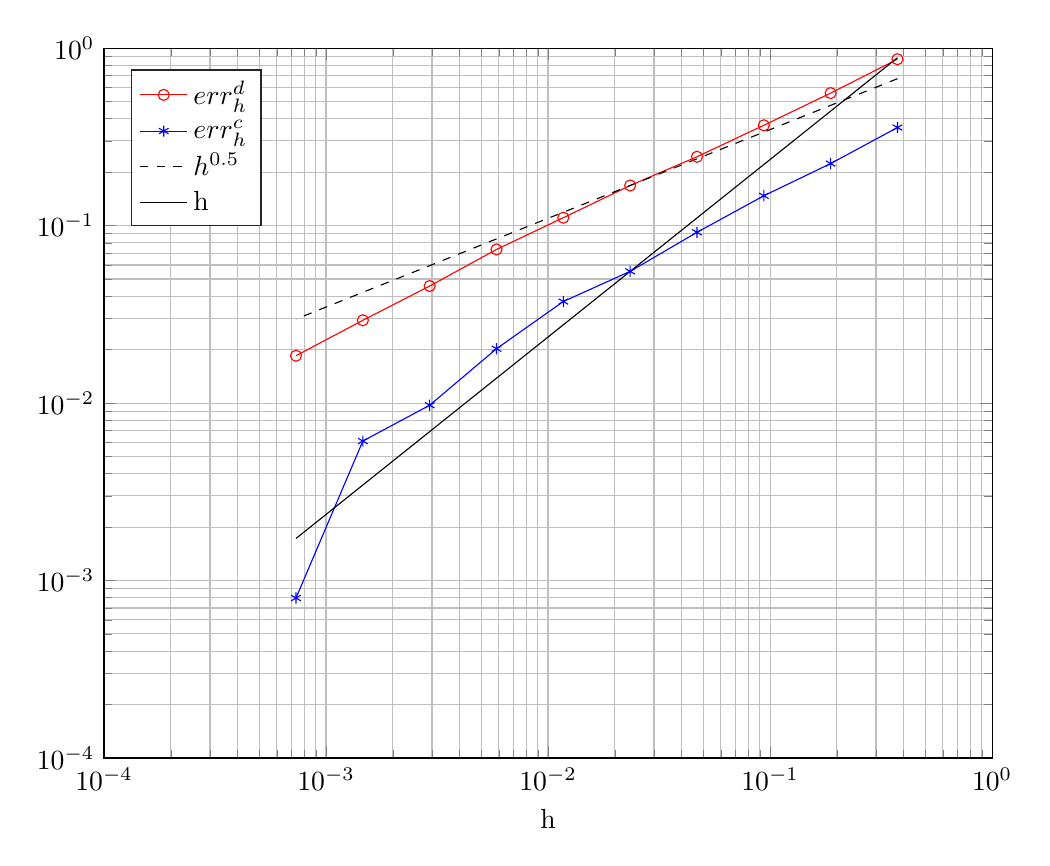
\begin{tikzpicture}

\begin{axis}[%
width=4.44in,
height=3.549in,
at={(0.745in,0.479in)},
scale only axis,
xmode=log,
xmin=0.0001,
xmax=1,
xminorticks=true,
xlabel={h},
xmajorgrids,
xminorgrids,
ymode=log,
ymin=0.0001,
ymax=1,
yminorticks=true,
ymajorgrids,
yminorgrids,
axis background/.style={fill=white},
legend style={at={(0.03,0.97)},anchor=north west,legend cell align=left,align=left,draw=white!15!black}
]
\addplot [color=red,solid,mark=o,mark options={solid}]
  table[row sep=crcr]{%
0.375	0.866448920874179\\
0.1875	0.558236420874179\\
0.09375	0.367633295874179\\
0.046875	0.244380170874179\\
0.0234375	0.168257514624179\\
0.01171875	0.110787592749179\\
0.005859375	0.0734094677491791\\
0.0029296875	0.0456410107179291\\
0.00146484375	0.0292624462648041\\
0.000732421875	0.0184820751710541\\
};
\addlegendentry{$\text{err}_\text{h}^\text{d}$};

\addplot [color=blue,solid,mark=asterisk,mark options={solid}]
  table[row sep=crcr]{%
0.375	0.357161420874179\\
0.1875	0.223680170874179\\
0.09375	0.147283295874179\\
0.046875	0.0916567333741791\\
0.0234375	0.0552278271241791\\
0.01171875	0.0373567333741791\\
0.005859375	0.0202379833741791\\
0.0029296875	0.0097233349366791\\
0.00146484375	0.00610927243667908\\
0.000732421875	0.000796943335116596\\
};
\addlegendentry{$\text{err}_\text{h}^\text{c}$};

\addplot [color=black,dashed]
  table[row sep=crcr]{%
0.375	0.673030058496717\\
0.1875	0.475904118305407\\
0.09375	0.336515029248358\\
0.046875	0.237952059152704\\
0.0234375	0.168257514624179\\
0.01171875	0.118976029576352\\
0.005859375	0.0841287573120896\\
0.0029296875	0.0594880147881759\\
0.00146484375	0.0420643786560448\\
0.000732421875	0.0297440073940879\\
};
\addlegendentry{$\text{h}^{\text{0.5}}$};

\addplot [color=black,solid]
  table[row sep=crcr]{%
0.375	0.883645233986866\\
0.1875	0.441822616993433\\
0.09375	0.220911308496716\\
0.046875	0.110455654248358\\
0.0234375	0.0552278271241791\\
0.01171875	0.0276139135620896\\
0.005859375	0.0138069567810448\\
0.0029296875	0.00690347839052239\\
0.00146484375	0.00345173919526119\\
0.000732421875	0.0017258695976306\\
};
\addlegendentry{h};

\end{axis}
\end{tikzpicture}% }  
        \caption{Reflecting boundary in $x = 1$}
        \label{fig:ReflectOneD}
    \end{subfigure}    
    \caption{Orders of convergence for DEM and CEM in the one-dimensional case.}
    \label{fig:OrdersOneD}
\end{figure}

\begin{figure}[t]
    \centering
    \begin{subfigure}{0.49\linewidth}
        \centering
        \resizebox{1\linewidth}{!}{% This file was created by matlab2tikz.
%
%The latest updates can be retrieved from
%  http://www.mathworks.com/matlabcentral/fileexchange/22022-matlab2tikz-matlab2tikz
%where you can also make suggestions and rate matlab2tikz.
%
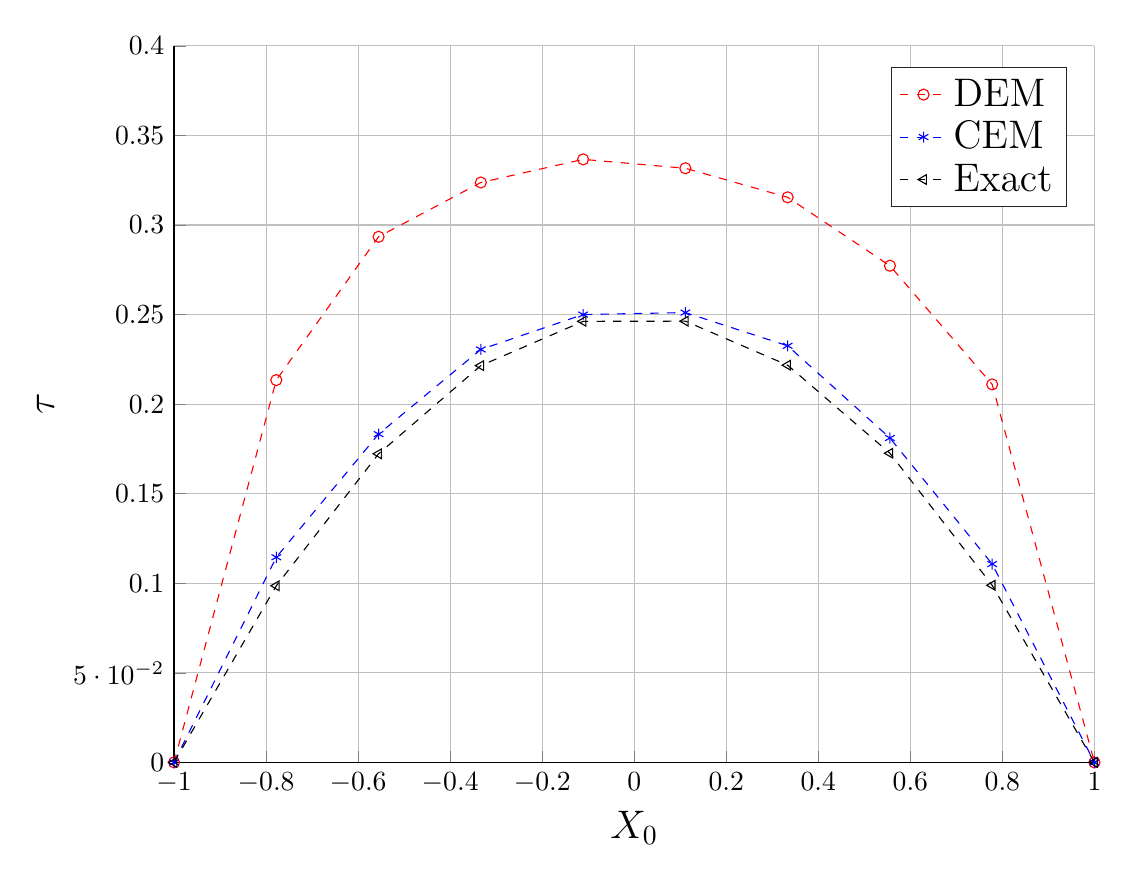
\begin{tikzpicture}

\begin{axis}[%
width=4.602in,
height=3.583in,
at={(0.772in,0.484in)},
scale only axis,
xmin=-1,
xmax=1,
xlabel={$X_0$},
xlabel style = {font = \Large},
xmajorgrids,
ymin=0,
ymax=0.4,
ylabel={$\tau$},
ylabel style = {font = \Large},
ymajorgrids,
axis background/.style={fill=white},
axis x line*=bottom,
axis y line*=left,
legend pos = north east,
legend style={legend cell align=left,align=left,draw=white!15!black,font=\Large}
]
\addplot [color=red,dashed,mark=o,mark options={solid}]
  table[row sep=crcr]{%
-1	0\\
-0.777777777777778	0.213421875\\
-0.555555555555556	0.2934140625\\
-0.333333333333333	0.3236953125\\
-0.111111111111111	0.336609375\\
0.111111111111111	0.331640625\\
0.333333333333333	0.315421875\\
0.555555555555556	0.2772421875\\
0.777777777777778	0.2110078125\\
1	0\\
};
\addlegendentry{DEM};

\addplot [color=blue,dashed,mark=asterisk,mark options={solid}]
  table[row sep=crcr]{%
-1	0\\
-0.777777777777778	0.114515625\\
-0.555555555555556	0.1832578125\\
-0.333333333333333	0.2305078125\\
-0.111111111111111	0.249984375\\
0.111111111111111	0.2510859375\\
0.333333333333333	0.232546875\\
0.555555555555556	0.181078125\\
0.777777777777778	0.11071875\\
1	0\\
};
\addlegendentry{CEM};

\addplot [color=black,dashed,mark=triangle,mark options={solid,rotate=90}]
  table[row sep=crcr]{%
-1	0\\
-0.777777777777778	0.0986011931395157\\
-0.555555555555556	0.172254291984329\\
-0.333333333333333	0.221472162307402\\
-0.111111111111111	0.246204174763737\\
0.111111111111111	0.2462957329545\\
0.333333333333333	0.221719125026098\\
0.555555555555556	0.172574095814315\\
0.777777777777778	0.0988572350577004\\
1	0\\
};
\addlegendentry{Exact};

\end{axis}
\end{tikzpicture}%
 }  
        \caption{Killing boundary in $x = 1$}
        \label{fig:ApproxOneD}
    \end{subfigure}
    \begin{subfigure}{0.49\linewidth}
        \centering
        \resizebox{1\linewidth}{!}{% This file was created by matlab2tikz.
%
%The latest updates can be retrieved from
%  http://www.mathworks.com/matlabcentral/fileexchange/22022-matlab2tikz-matlab2tikz
%where you can also make suggestions and rate matlab2tikz.
%
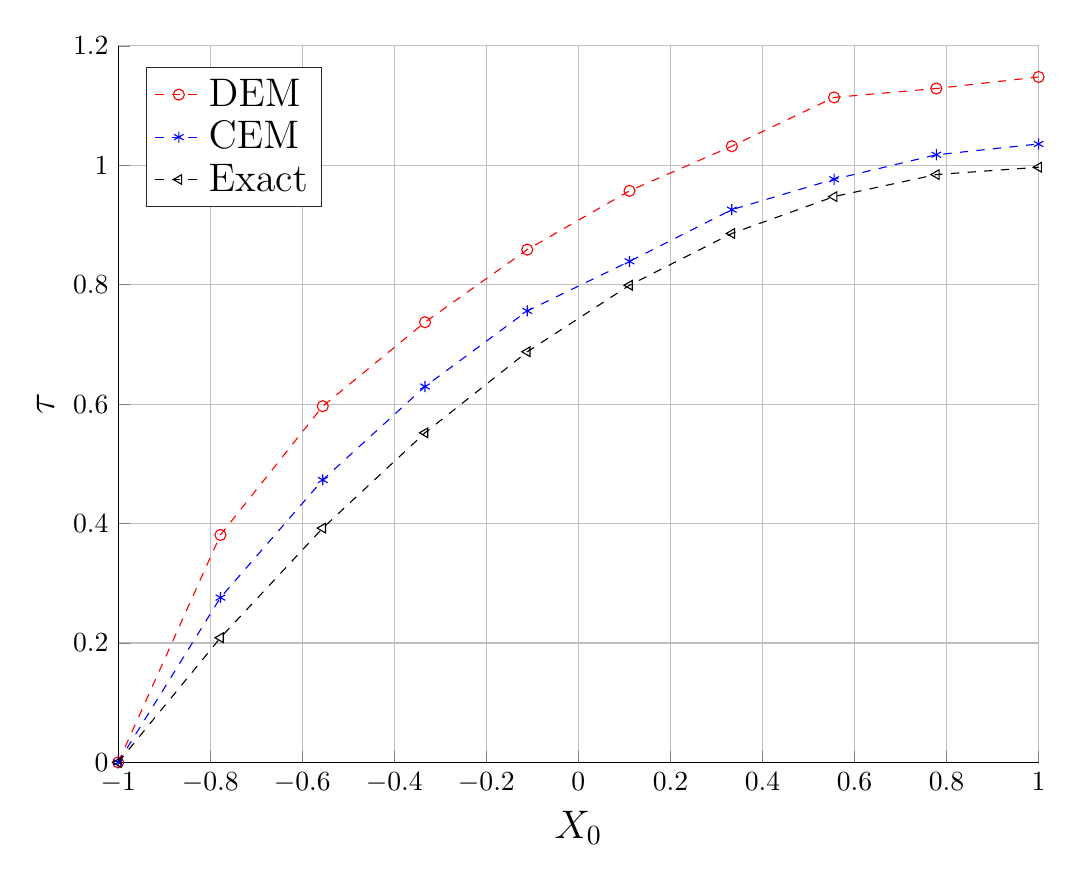
\begin{tikzpicture}

\begin{axis}[%
width=4.602in,
height=3.583in,
at={(0.772in,0.484in)},
scale only axis,
xmin=-1,
xmax=1,
xlabel={$X_0$},
xlabel style={font=\Large},
xmajorgrids,
ymin=0,
ymax=1.2,
ylabel={$\tau$},
ylabel style={font=\Large},
ymajorgrids,
axis background/.style={fill=white},
axis x line*=bottom,
axis y line*=left,
legend style={at={(0.03,0.97)},anchor=north west,legend cell align=left,align=left,draw=white!15!black,font=\Large}
]
\addplot [color=red,dashed,mark=o,mark options={solid}]
  table[row sep=crcr]{%
-1	0\\
-0.777777777777778	0.3809765625\\
-0.555555555555556	0.5964609375\\
-0.333333333333333	0.73715625\\
-0.111111111111111	0.8587265625\\
0.111111111111111	0.9571171875\\
0.333333333333333	1.031859375\\
0.555555555555556	1.113609375\\
0.777777777777778	1.1285390625\\
1	1.1478046875\\
};
\addlegendentry{DEM};

\addplot [color=blue,dashed,mark=asterisk,mark options={solid}]
  table[row sep=crcr]{%
-1	0\\
-0.777777777777778	0.275953125\\
-0.555555555555556	0.4729921875\\
-0.333333333333333	0.629484375\\
-0.111111111111111	0.7560703125\\
0.111111111111111	0.8390625\\
0.333333333333333	0.9255703125\\
0.555555555555556	0.976546875\\
0.777777777777778	1.017515625\\
1	1.035609375\\
};
\addlegendentry{CEM};

\addplot [color=black,dashed,mark=triangle,mark options={solid,rotate=90}]
  table[row sep=crcr]{%
-1	0\\
-0.777777777777778	0.208777054487475\\
-0.555555555555556	0.392333503315235\\
-0.333333333333333	0.551939853868488\\
-0.111111111111111	0.687661056545228\\
0.111111111111111	0.79906851214989\\
0.333333333333333	0.885727939207175\\
0.555555555555556	0.947463001823471\\
0.777777777777778	0.984384604394486\\
1	0.996687130893952\\
};
\addlegendentry{Exact};

\end{axis}
\end{tikzpicture}%
 }  
        \caption{Reflecting boundary in $x = 1$}
        \label{fig:ApproxOneD}
    \end{subfigure}    
    \caption{Approximation of $\tau$ for the discrete and continuous EM method in the one-dimensional case.}
    \label{fig:ApproxOneD}
\end{figure}

\begin{figure}[t]
        \centering
        \resizebox{0.6\linewidth}{!}{% This file was created by matlab2tikz.
%
%The latest updates can be retrieved from
%  http://www.mathworks.com/matlabcentral/fileexchange/22022-matlab2tikz-matlab2tikz
%where you can also make suggestions and rate matlab2tikz.
%
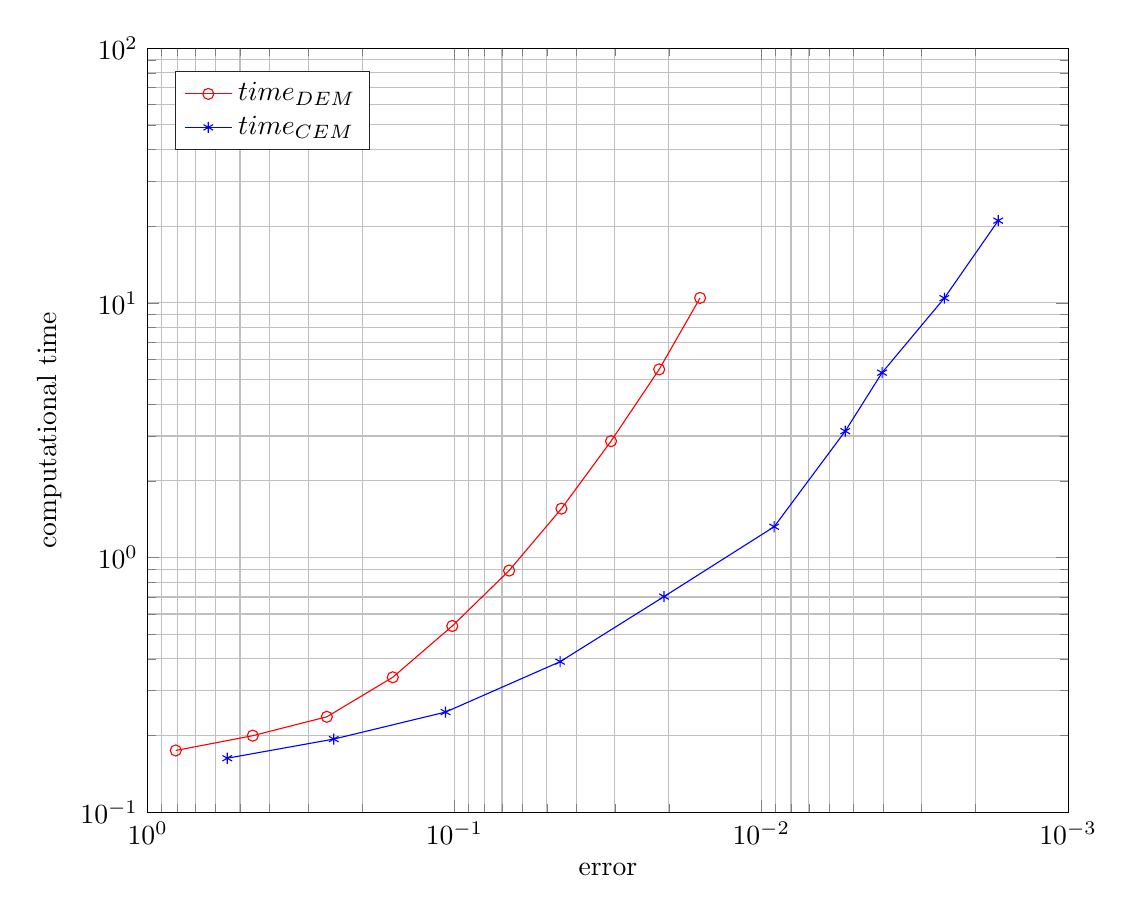
\begin{tikzpicture}

\begin{axis}[%
width=4.602in,
height=3.82in,
at={(0.772in,0.516in)},
scale only axis,
x dir=reverse,
xmode=log,
xmin=0.001,
xmax=1,
xminorticks=true,
xlabel={error},
xmajorgrids,
xminorgrids,
ymode=log,
ymin=0.1,
ymax=100,
yminorticks=true,
ylabel={computational time},
ymajorgrids,
yminorgrids,
axis background/.style={fill=white},
legend style={at={(0.03,0.97)},anchor=north west,legend cell align=left,align=left,draw=white!15!black}
]
\addplot [color=red,solid,mark=o,mark options={solid}]
  table[row sep=crcr]{%
0.809808666527388	0.174713\\
0.454308666527388	0.199743\\
0.260652416527388	0.23684\\
0.158902416527388	0.338576\\
0.101648510277388	0.538431\\
0.0663692134023876	0.888358\\
0.0448057368398877	1.555625\\
0.0308814204336377	2.863223\\
0.0215156977773877	5.478668\\
0.0158268550039502	10.454508\\
};
\addlegendentry{$\text{time}_{\text{DEM}}$};

\addplot [color=blue,solid,mark=asterisk,mark options={solid}]
  table[row sep=crcr]{%
0.550433666527388	0.162876\\
0.247433666527388	0.193649\\
0.106918041527388	0.247227\\
0.0452461665273877	0.390013\\
0.0207461665273877	0.702369\\
0.00907819777738766	1.320507\\
0.00532429152738766	3.134469\\
0.00403864699613767	5.317267\\
0.00253132277738766	10.432115\\
0.00168928176176265	21.021666\\
};
\addlegendentry{$\text{time}_{\text{CEM}}$};

\end{axis}
\end{tikzpicture}% }  
        \caption{error vs work plot for DEM and CEM.}
        \label{fig:CompTime}
\end{figure}


\vspace{2mm}
\noindent\textbf{Rough case.} We consider the same domain $D$ as above, $T = 5$ and $g = \sigma = 3$. We consider $V$ to be piecewise linear, so that $f = -dV$ is piecewise constant. In particular, we choose the following form for $V$
\begin{equation}\label{eq:FunctionsOneDRough}
V = 0.1 
\left \{
\begin{aligned}
	 -2x -1&, && x < -0.5, \\
	 4x + 2&, && -0.5 \leq x < 0, \\
	 -2x + 2&, &&  0 \leq x < 0.5, \\
	 4x - 1&, && x \geq 0.5.
\end{aligned} \right .
\end{equation}
This is a linear interpolation of the function $V$ we used in the smooth case above in the points $\{-1,-0.5,0,0.5,1\}$. This case is of particular interest, since if the function $f$ is the result of a numerical method on a $PDE$, it could not be smooth as in the previous case. We perform DEM and CEM with the same parameters as before, \textit{i.e.}, $M = 10000, N = 2^i,i=3,\dots,12$. In Figure \ref{fig:OrdersOneDRough} it is possible to remark that the rate of convergence of DEM is unvaried with respect to the previous case. The CEM method experiences a slight decrease in the order of convergence with respect to the smooth case.


\begin{figure}[t]
    \centering
    \begin{subfigure}{0.49\linewidth}
        \centering
        \resizebox{1\linewidth}{!}{% This file was created by matlab2tikz.
%
%The latest updates can be retrieved from
%  http://www.mathworks.com/matlabcentral/fileexchange/22022-matlab2tikz-matlab2tikz
%where you can also make suggestions and rate matlab2tikz.
%
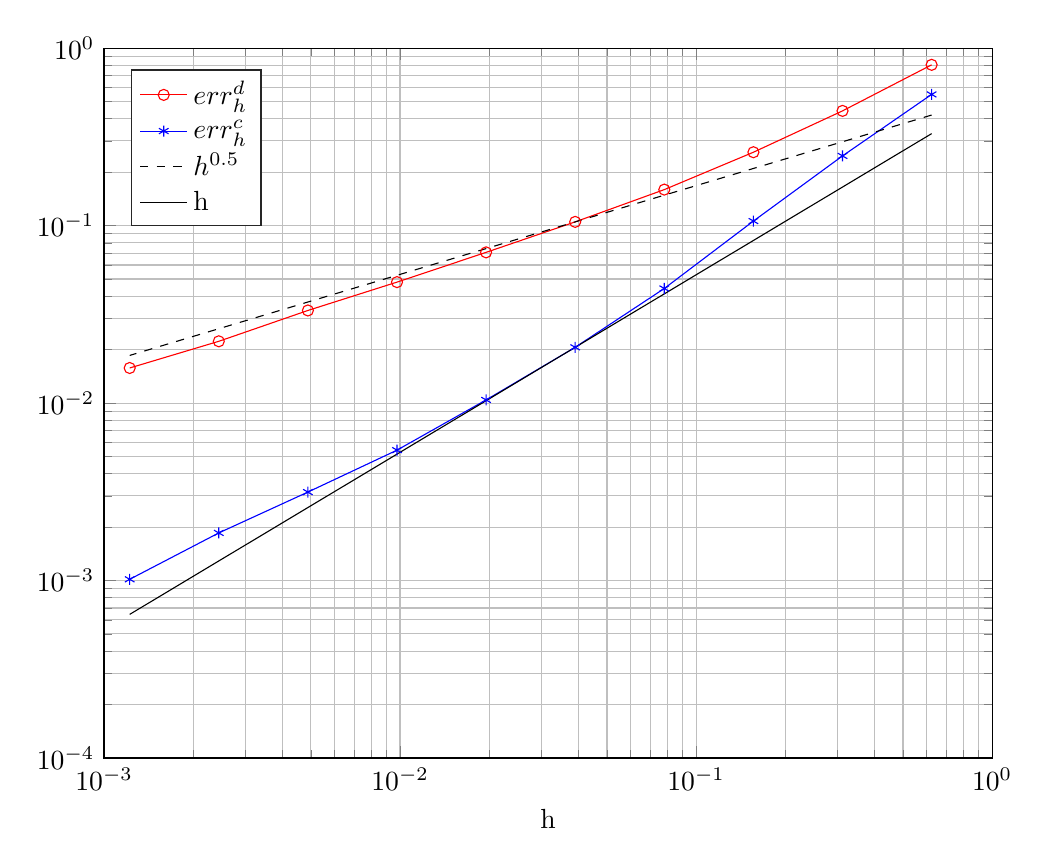
\begin{tikzpicture}

\begin{axis}[%
width=4.44in,
height=3.549in,
at={(0.745in,0.479in)},
scale only axis,
xmode=log,
xmin=0.001,
xmax=1,
xminorticks=true,
xlabel={h},
xmajorgrids,
xminorgrids,
ymode=log,
ymin=0.0001,
ymax=1,
yminorticks=true,
ymajorgrids,
yminorgrids,
axis background/.style={fill=white},
legend style={at={(0.03,0.97)},anchor=north west,legend cell align=left,align=left,draw=white!15!black}
]
\addplot [color=red,solid,mark=o,mark options={solid}]
  table[row sep=crcr]{%
0.625	0.805508168582389\\
0.3125	0.443133168582389\\
0.15625	0.259164418582389\\
0.078125	0.159539418582389\\
0.0390625	0.104953481082389\\
0.01953125	0.0706722310823888\\
0.009765625	0.0480316060823888\\
0.0048828125	0.0332552388948888\\
0.00244140625	0.0222842916292638\\
0.001220703125	0.0157625631136388\\
};
\addlegendentry{$\text{err}_\text{h}^\text{d}$};

\addplot [color=blue,solid,mark=asterisk,mark options={solid}]
  table[row sep=crcr]{%
0.625	0.548758168582389\\
0.3125	0.247101918582389\\
0.15625	0.106070668582389\\
0.078125	0.0442191060823888\\
0.0390625	0.0206175435823888\\
0.01953125	0.0104124654573888\\
0.009765625	0.00542809045738883\\
0.0048828125	0.00315025842613884\\
0.00244140625	0.00185411584801383\\
0.001220703125	0.00101573694176384\\
};
\addlegendentry{$\text{err}_\text{h}^\text{c}$};

\addplot [color=black,dashed]
  table[row sep=crcr]{%
0.625	0.419813924329555\\
0.3125	0.296853272729965\\
0.15625	0.209906962164778\\
0.078125	0.148426636364982\\
0.0390625	0.104953481082389\\
0.01953125	0.0742133181824912\\
0.009765625	0.0524767405411944\\
0.0048828125	0.0371066590912456\\
0.00244140625	0.0262383702705972\\
0.001220703125	0.0185533295456228\\
};
\addlegendentry{$\text{h}^{\text{0.5}}$};

\addplot [color=black,solid]
  table[row sep=crcr]{%
0.625	0.329880697318221\\
0.3125	0.164940348659111\\
0.15625	0.0824701743295553\\
0.078125	0.0412350871647776\\
0.0390625	0.0206175435823888\\
0.01953125	0.0103087717911944\\
0.009765625	0.0051543858955972\\
0.0048828125	0.0025771929477986\\
0.00244140625	0.0012885964738993\\
0.001220703125	0.000644298236949651\\
};
\addlegendentry{h};

\end{axis}
\end{tikzpicture}% }  
        \caption{Killing boundary in $x = 1$}
        \label{fig:KillOneDRough}
    \end{subfigure}
    \begin{subfigure}{0.49\linewidth}
        \centering
        \resizebox{1\linewidth}{!}{% This file was created by matlab2tikz.
%
%The latest updates can be retrieved from
%  http://www.mathworks.com/matlabcentral/fileexchange/22022-matlab2tikz-matlab2tikz
%where you can also make suggestions and rate matlab2tikz.
%
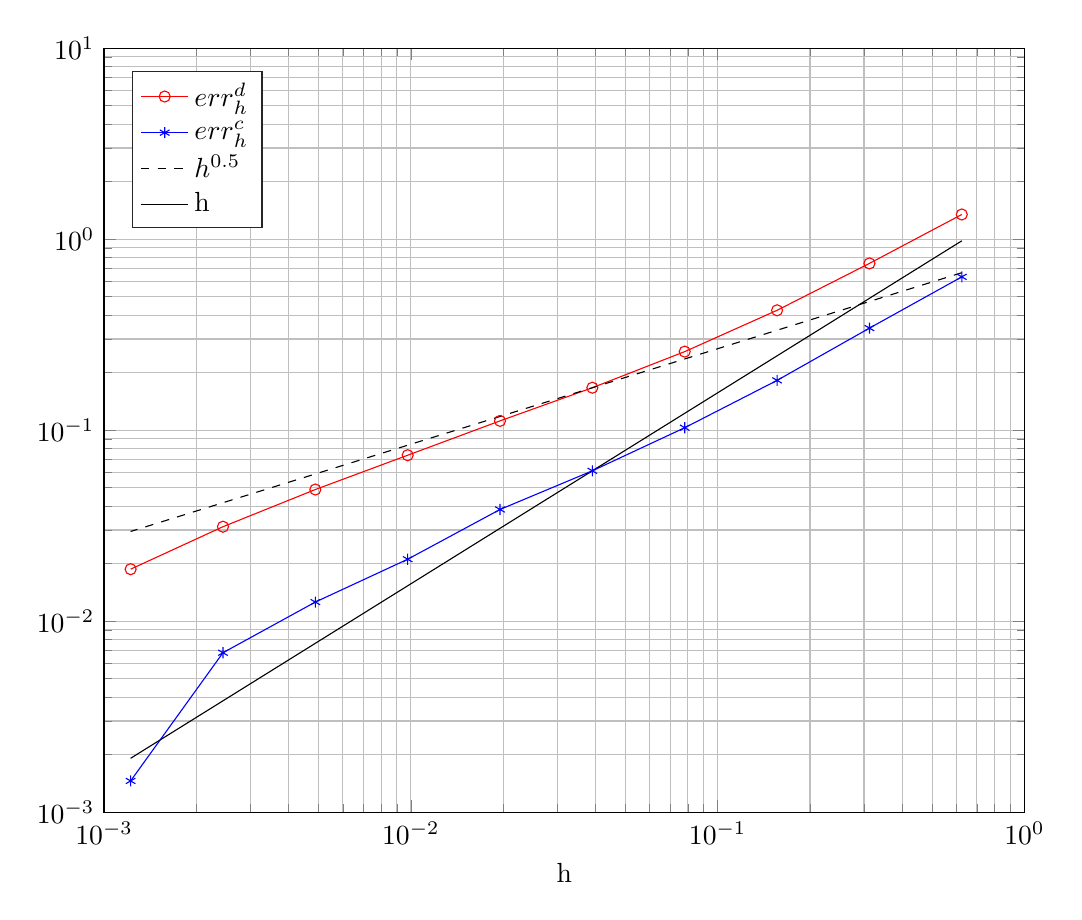
\begin{tikzpicture}

\begin{axis}[%
width=4.602in,
height=3.82in,
at={(0.772in,0.516in)},
scale only axis,
xmode=log,
xmin=0.001,
xmax=1,
xminorticks=true,
xlabel={h},
xmajorgrids,
xminorgrids,
ymode=log,
ymin=0.001,
ymax=10,
yminorticks=true,
ymajorgrids,
yminorgrids,
axis background/.style={fill=white},
legend style={at={(0.03,0.97)},anchor=north west,legend cell align=left,align=left,draw=white!15!black}
]
\addplot [color=red,solid,mark=o,mark options={solid}]
  table[row sep=crcr]{%
0.625	1.34651720868191\\
0.3125	0.746735958681911\\
0.15625	0.424189083681911\\
0.078125	0.257767208681911\\
0.0390625	0.166806271181911\\
0.01953125	0.111831661806911\\
0.009765625	0.0739322477444107\\
0.0048828125	0.0488814664944107\\
0.00244140625	0.0312279020412857\\
0.001220703125	0.0187126432522232\\
};
\addlegendentry{$\text{err}_\text{h}^\text{d}$};

\addplot [color=blue,solid,mark=asterisk,mark options={solid}]
  table[row sep=crcr]{%
0.625	0.634767208681911\\
0.3125	0.342173458681911\\
0.15625	0.182251583681911\\
0.078125	0.102985958681911\\
0.0390625	0.0612633024319106\\
0.01953125	0.0384371305569107\\
0.009765625	0.0210972868069106\\
0.0048828125	0.0125884977444107\\
0.00244140625	0.00683532391628566\\
0.001220703125	0.00145739422878566\\
};
\addlegendentry{$\text{err}_\text{h}^\text{c}$};

\addplot [color=black,dashed]
  table[row sep=crcr]{%
0.625	0.667225084727643\\
0.3125	0.471799381988685\\
0.15625	0.333612542363821\\
0.078125	0.235899690994342\\
0.0390625	0.166806271181911\\
0.01953125	0.117949845497171\\
0.009765625	0.0834031355909553\\
0.0048828125	0.0589749227485856\\
0.00244140625	0.0417015677954777\\
0.001220703125	0.0294874613742928\\
};
\addlegendentry{$\text{h}^{\text{0.5}}$};

\addplot [color=black,solid]
  table[row sep=crcr]{%
0.625	0.98021283891057\\
0.3125	0.490106419455285\\
0.15625	0.245053209727643\\
0.078125	0.122526604863821\\
0.0390625	0.0612633024319106\\
0.01953125	0.0306316512159553\\
0.009765625	0.0153158256079777\\
0.0048828125	0.00765791280398883\\
0.00244140625	0.00382895640199441\\
0.001220703125	0.00191447820099721\\
};
\addlegendentry{h};

\end{axis}
\end{tikzpicture}% }  
        \caption{Reflecting boundary in $x = 1$}
        \label{fig:ReflectOneDRough}
    \end{subfigure}    
    \caption{Orders of convergence for DEM and CEM in the one-dimensional case with $f$ piecewise constant.}
    \label{fig:OrdersOneDRough}
\end{figure}

